%\documentclass{article}
%\usepackage{tikz}
%\begin{document}


    	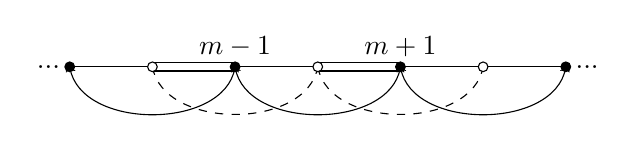
\begin{tikzpicture}[scale=.7]
    		\newcommand{\orig}{-1.5}
    		\newcommand{\trans}{1.5}
    		\newcommand{\vertspac}{-2.}
    		\newcommand{\vertsize}{0} % vertical span of the rectangles
    		\newcommand{\del}{.2}
    		\newcommand{\rad}{2.5pt} % radii of the circles

    		
    		% set the style of the strong bonds
    		\tikzset{
    			strong/.style={
    				double,
    				double distance=\rad,
    				line width=0.5pt
    				}
    		}
			% arrows
			\path[<->] (\orig+0*\trans,0) edge[bend right = 80] (\orig+2*\trans,0);
			\path[<->] (\orig+2*\trans,0) edge[bend right = 80] (\orig+4*\trans,0);
			\path[<->] (\orig+4*\trans,0) edge[bend right = 80] (\orig+6*\trans,0);
			%\path[<->] (\orig+6*\trans,0) edge[bend right = 80] (\orig+8*\trans,0);			
			
    		% dotted arrows
			\path[-, dashed] (\orig+1*\trans,0) edge[bend right = 80] (\orig+3*\trans,0);
			\path[-, dashed] (\orig+3*\trans,0) edge[bend right = 80] (\orig+5*\trans,0);
			%\path[-, dashed] (\orig+5*\trans,0) edge[bend right = 80] (\orig+7*\trans,0);
    	
    		% bonds 
        	\draw[-] (\orig, 0)  node [left] {...}  -- (\orig+\trans, 0) node [midway, below] {};
			\draw[strong] (\orig+\trans,0) -- (\orig+2*\trans,0) node [midway, below] {};
			\draw[-] (\orig+2*\trans,0) -- (\orig+3*\trans,0) node [midway, below] {};	
			\draw[strong] (\orig+3*\trans,0) -- (\orig+4*\trans,0) node [midway, below] {};
			\draw[-] (\orig+4*\trans,0) -- (\orig+5*\trans,0) node [midway, below] {};
			\draw[-] (\orig+5*\trans,0) -- (\orig+6*\trans,0) node [right] {...} node [midway, below] {};
			%\draw[strong] (\orig+6*\trans,0) -- (\orig+7*\trans,0) node [midway, below] {};
			%\draw[-] (\orig+7*\trans,0) -- (\orig+8*\trans,0) node [right] {...} node [midway, below] {};
    	
    		% sites
			\filldraw (\orig+0*\trans,0) circle (\rad);% node [below] {$h=0$} node [above] {$\psi=1$};
			\filldraw [fill=white] (\orig+1*\trans,0) circle (\rad);% node [below] {};
			\filldraw (\orig+2*\trans,0) circle (\rad) node [above] {$m-1$};
			\filldraw [fill=white] (\orig+3*\trans,0) circle (\rad);% node [below] {};
			\filldraw (\orig+4*\trans,0) circle (\rad) node [above] {$m+1$};% node [above] {$\psi = \rho^2$};
			\filldraw [fill=white] (\orig+5*\trans,0) circle (\rad);% node [below] {};
			\filldraw (\orig+6*\trans,0) circle (\rad);% node [below] {$h=2$} node [above] {$\psi = \rho^2$};
			%\filldraw [fill=white] (\orig+7*\trans,0) circle (\rad);% node [below] {};
			%\filldraw (\orig+8*\trans,0) circle (\rad);% node [below] {$h=1$} node [above] {$\psi = \rho$};
		\end{tikzpicture}

%\end{document}